\subsection{Fuzzy Network}

\subsubsection{Scelta del modello}
Il concetto base della logica fuzzy è quello di mappare uno spazio di ingresso in uno spazio di uscita sfruttando un elenco di relazioni if-then chiamate regole.

Tali regole si riferiscono a variabili e ad aggettivi che le descrivono. Prima di poter costruire un sistema che interpreti le regole, è necessario definire tutti i termini che si pensa di utilizzare e gli aggettivi che li descrivono.

Il Fuzzy Logic Toolbox (fuzzy) di Matlab permette di creare due tipi di Fuzzy Inference Systems (FIS) che si differenziano per il modo in cui le uscite sono determinate:

\begin{itemize}
  \item Mamdani
  \item Sugeno
\end{itemize}

Nel seguito faremo riferimento ad un FIS Mamdani-type completamente definito sfruttando la GUI proposta da Matlab dove si è scelto di mantenere le impostazioni di default per le principali funzioni logiche.

Una fase preliminare importante consiste nel valutare e selezionare, in base ai dati forniti, le variabili di input e di output.

Per quanto riguarda gli input, ad esempio, la suddivisione tra giorno festivo e giorno feriale non può essere rappresentata utilizzando un modello fuzzy in quanto la suddetta suddivisione è netta e solo la creazione di 2 modelli distinti permette di tenerne conto.

Per lo stesso motivo considereremo i vari giorni della settimana come equivalenti, eccezion fatta per i giorni festivi, escludendo così anche questa componente dagli ingressi.

In ingresso al sistema perciò avremo soltanto due variabili, l’ora del giorno e l’irraggiamento esterno, in quanto i dati forniti non giustificano l’utilizzo di nessun’altra variabile che andrebbe soltanto a complicare il modello.

Si definirà un FIS per ogni variabile di uscita del problema in modo tale da poter ottimizzare il modello su tale output; avremo quindi un totale di quattro sistemi, rispettivamente, per la predizione di:

\begin{itemize}
  \item Energia consumata nei giorni festivi;
  \item Energia consumata nei giorni feriali;
  \item Luminosità misurata nei giorni festivi;
  \item Luminosità misurata nei giorni feriali (nel seguito si farà riferimento a questo scenario nell'illustrazione del procedimento utilizzato per la realizzazione del modello Fuzzy).
\end{itemize}


\subsubsection{Definizione delle MFs}
In ingresso al sistema avremo perciò, come discusso precedentemente, soltanto due variabili, l'ora del giorno e l'irraggiamento.

Il modello avrà la seguente struttura:

\begin{figure}
  \centering
  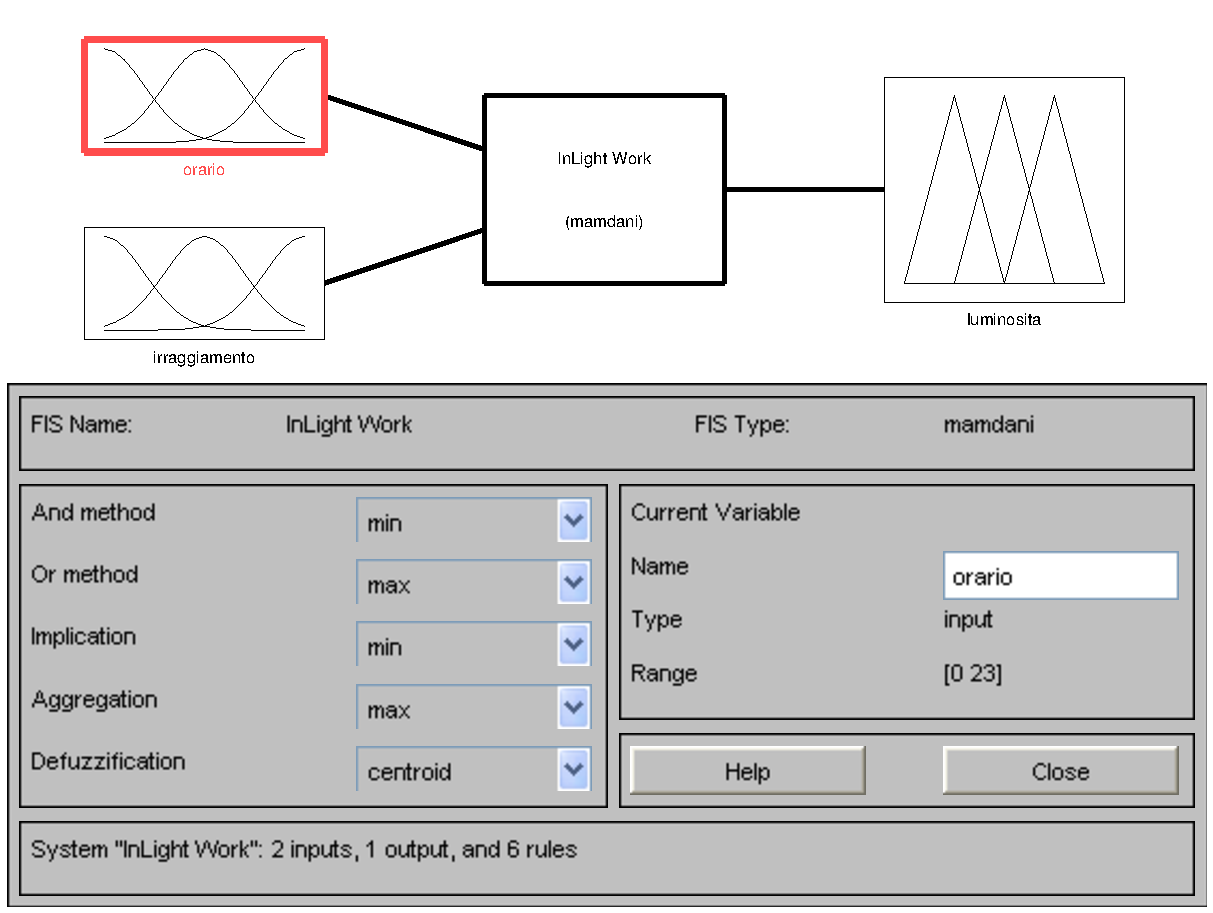
\includegraphics[scale=0.5]{images/fuzzy/modello_fuzzy_luminosita.pdf}
  \caption{Modello fuzzy luminosità}
\end{figure}

A questo punto è necessario analizzare ogni variabile per poter definire il suo insieme di valori significativi e successivamente le sue MFs.

Per quanto riguarda l'ora sono stati scelti cinque elementi lessicali (Notte, Prima Mattina, Mattina, Pomeriggio, Sera) che rappresentino gli insiemi fuzzy; le relative funzioni di appartenenza risulteranno:

\begin{figure}
  \centering
  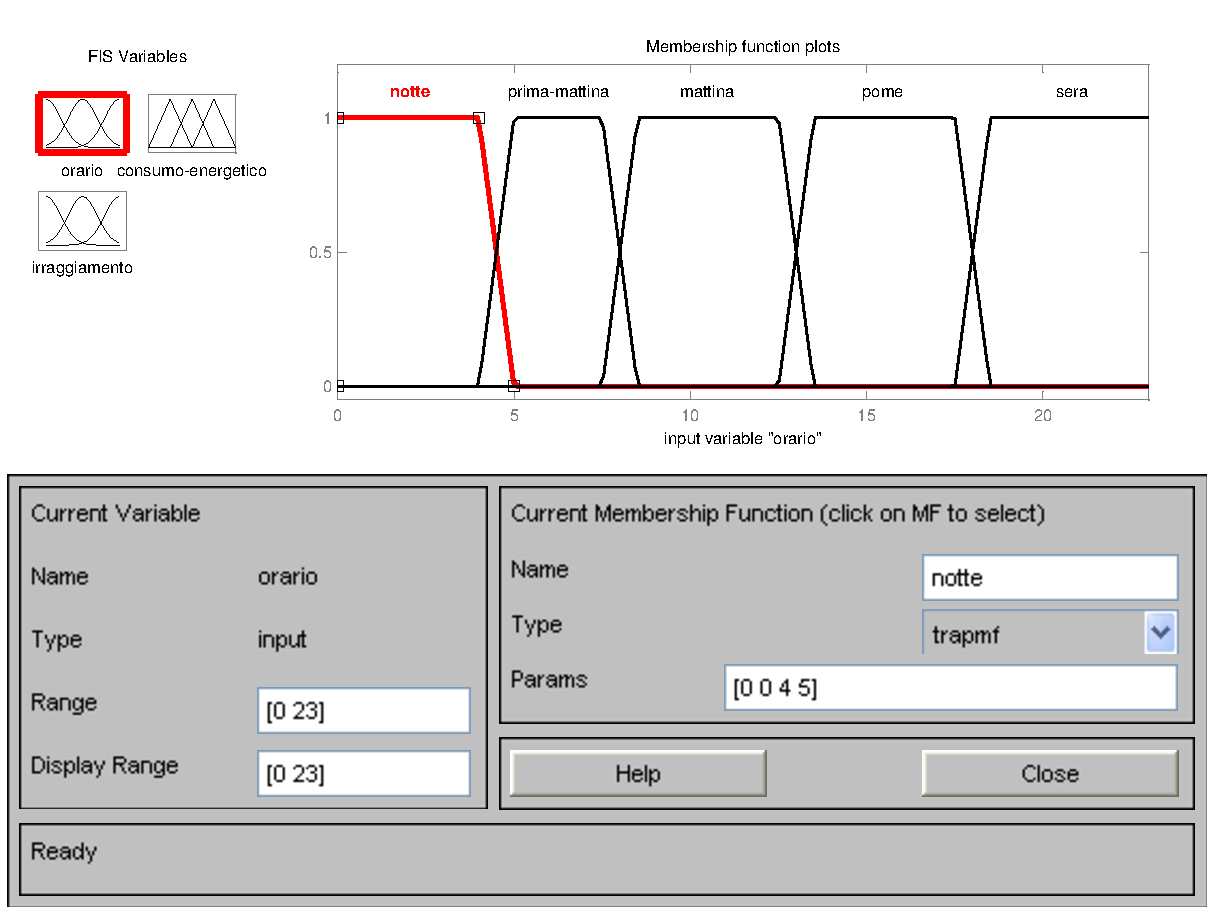
\includegraphics[scale=0.5]{images/fuzzy/variabile_orario.pdf}
  \caption{Variabile orario}
\end{figure}

Passando ora ad analizzare l'irraggiamento, attraverso lo studio dei dati forniti e del range di valori entro i quali si collocano, gli elementi lessicali sono quattro ({\em Basso, Medio, Alto, Molto Alto}) e le funzioni di appartenenza saranno:

\begin{figure}
  \centering
  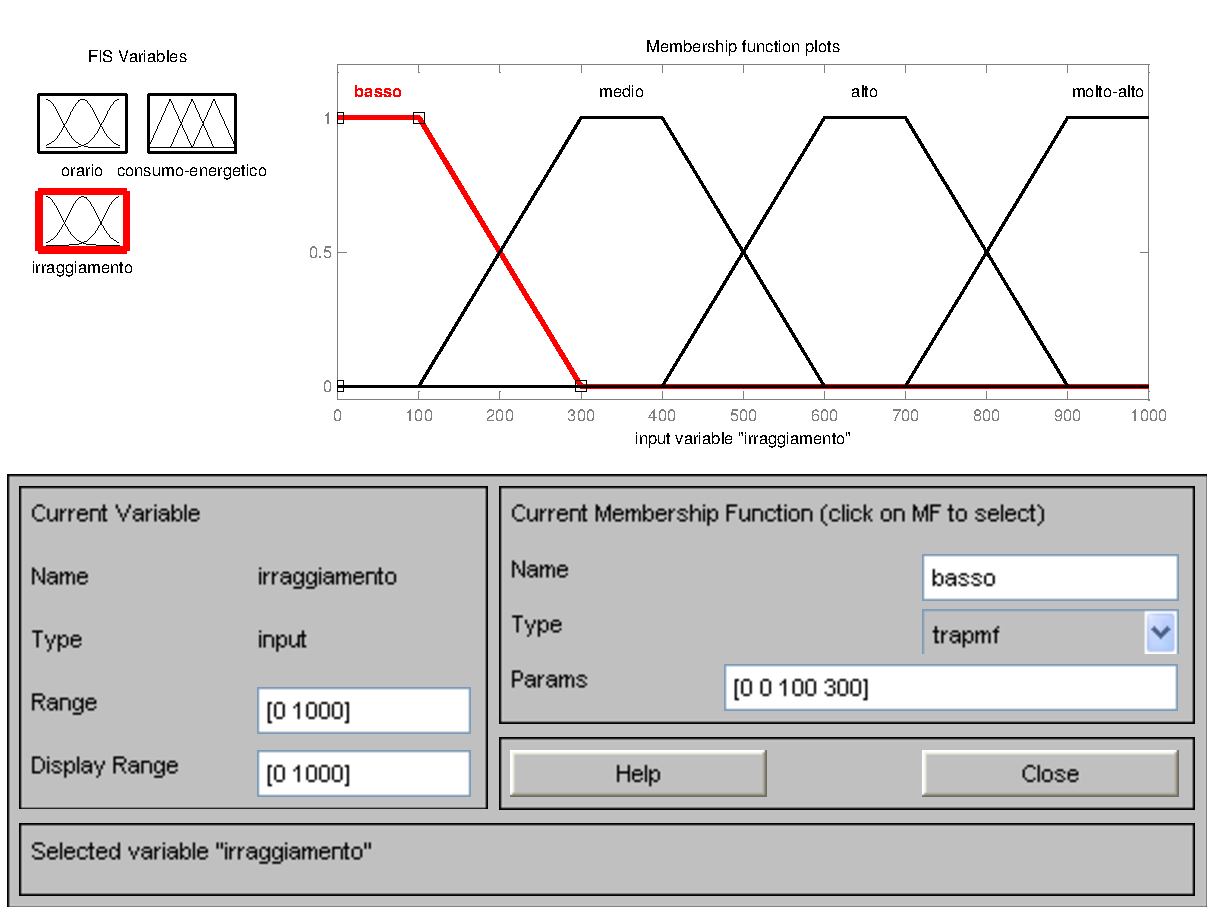
\includegraphics[scale=0.5]{images/fuzzy/variabile_irraggiamento.pdf}
  \caption{Variabile irraggiamento}
\end{figure}

Si possono ottenere con gli stessi ragionamenti risultati simili anche per la Luminosità:

\begin{figure}[htbp]
  \centering
  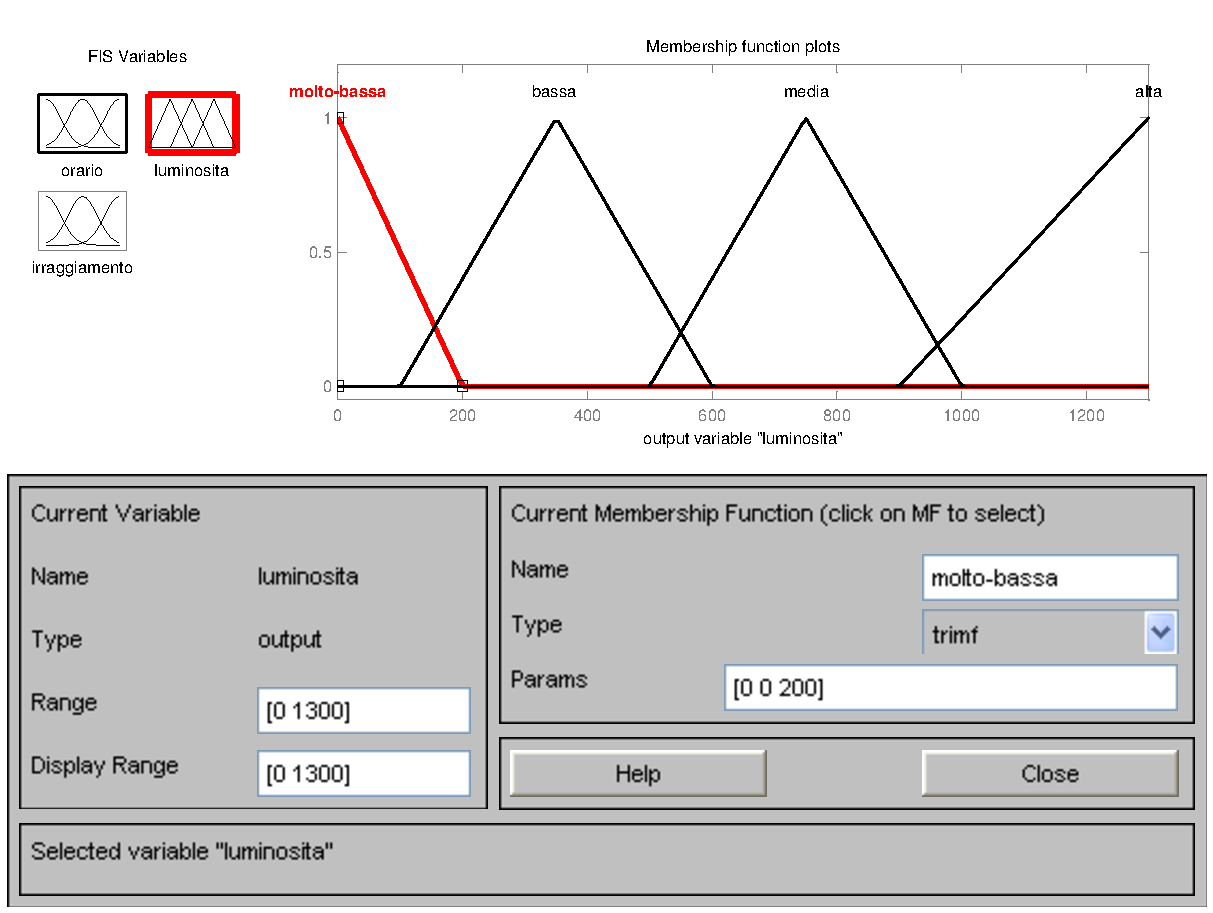
\includegraphics[scale=0.5]{images/fuzzy/variabile_luminosita.pdf}
  \caption{Variabile luminosità}
\end{figure}


\subsubsection{Definizione delle regole}
Non possedendo un'esperienza sufficiente nel campo dell'illuminazione per poter definire delle regole generali per il sistema fuzzy in esame, verranno estrapolate dai dati in nostro possesso le regole valide per il modello.

Nello specifico sono state ricavate le seguenti:

\begin{figure}[htbp]
  \centering
  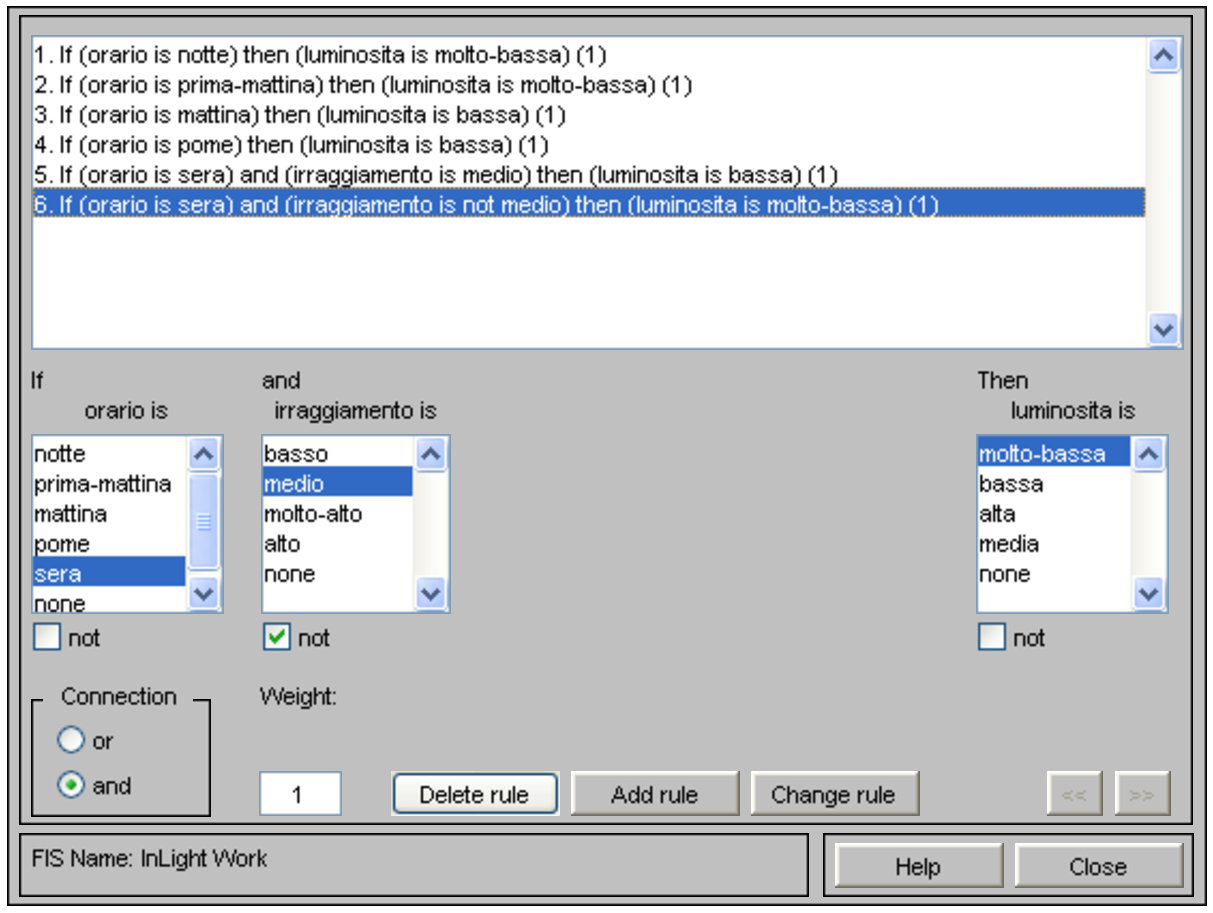
\includegraphics[scale=0.5]{images/fuzzy/regole_luminosita.pdf}
  \caption{Regole luminosità}
\end{figure}

A questo punto il FIS è completamente definita e si possono visualizzare le regole tramite il “Rule Viewer” e la curva tridimensionale che lega l'uscita ai due ingressi nel “Surface Viewer”:

\begin{figure}[htbp]
  \centering
  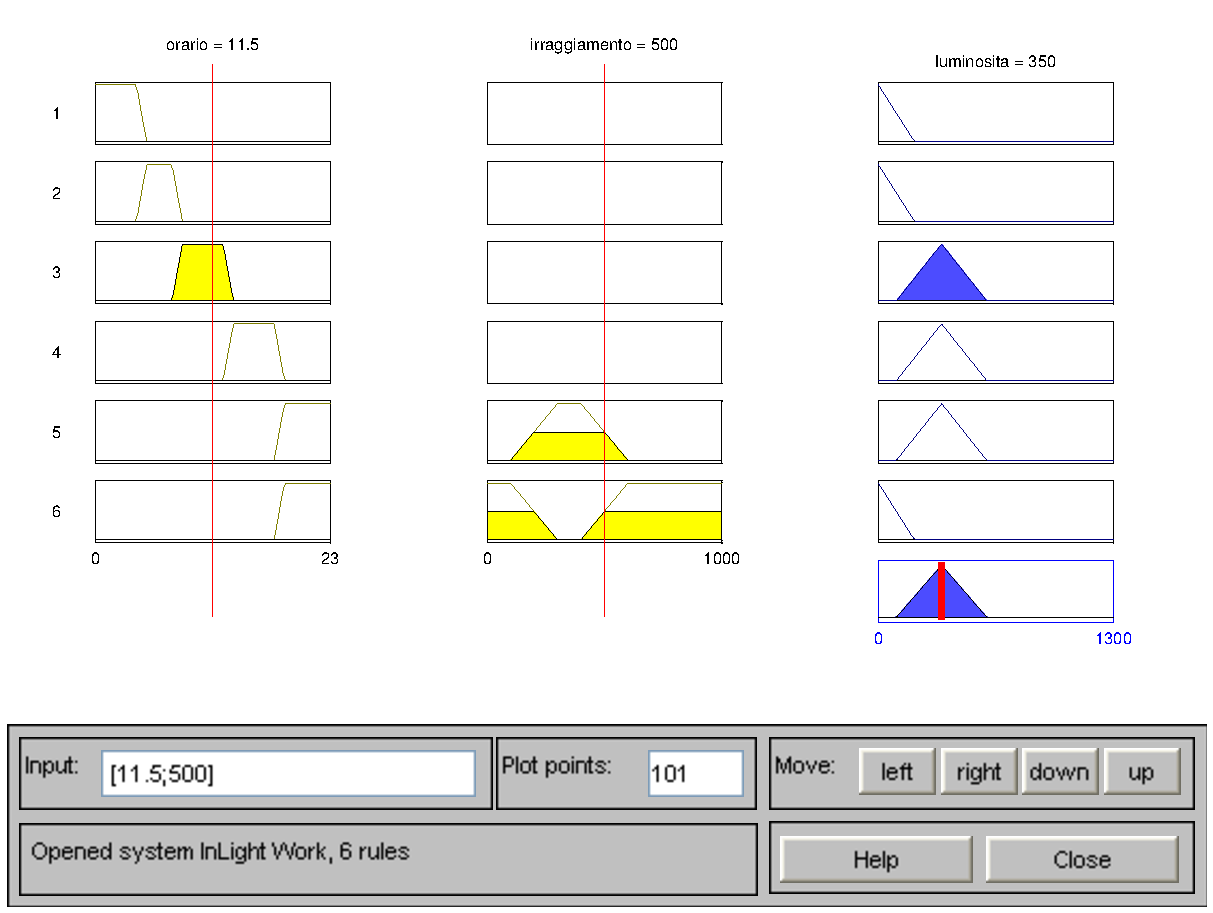
\includegraphics[scale=0.5]{images/fuzzy/regole_luminosita_rule_view.pdf}
  \caption{Regole luminosità rule view}
\end{figure}
\begin{figure}[htbp]
  \centering
  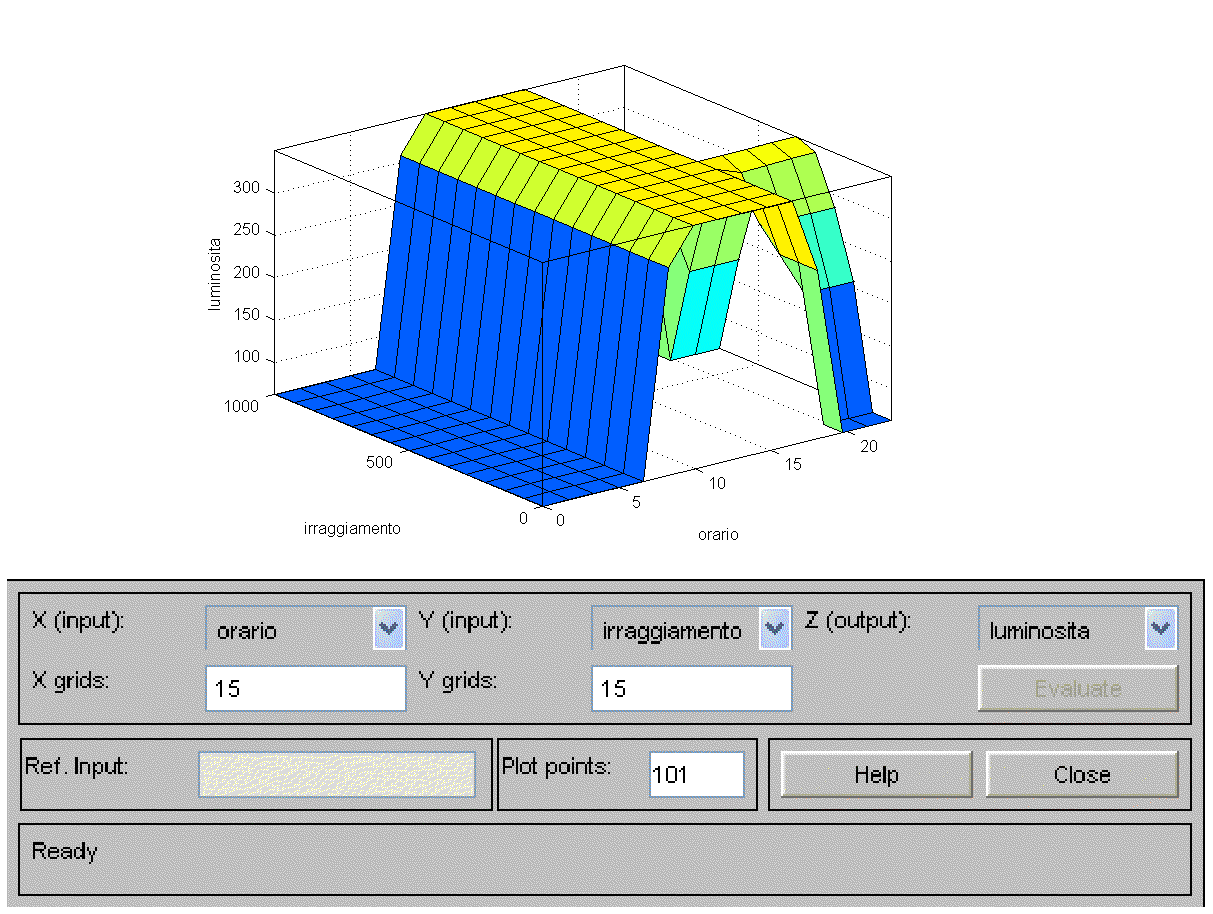
\includegraphics[scale=0.5]{images/fuzzy/regole_luminosita_surface_view.pdf}
  \caption{Regole luminosità surface view}
\end{figure}


\subsubsection{Manipolazione e studio dei risultati}
Una volta che il FIS è completamente definito deve essere valutato per testarne l'attendibilità.

Si utilizzerà perciò il comando Matlab “evalfis” assegnando in ingresso una coppia di vettori contenenti rispettivamente tutti i campioni forniti per ora e irraggiamento ( ovvero i due input del modello).

Il risultato fornito da evalfis sarà un vettore di valori crisp in cui l'i-esimo elemento rappresenta la Luminosità che il sistema fuzzy calcola per l'i-esima coppia in ingresso.

Si procede quindi alla fuzzificazione dei risultati forniti dal sistema e della luminosità presente nei dati. Confrontando i vettori si ottiene la percentuale di successi (hit), valore che può essere utilizzato come parametro prestazionale del sistema.

Per il caso in esame si ha una corrispondenza per 802 campioni, ovvero successo nell'80\% dei campioni.
\begin{table}
  \caption{Risultati}
  \centering
	\begin{tabular}{lr}
		\toprule
      \# di Entry & $1005$ \\
			\# di Hit   & $802$ \\
		\midrule
			& $80\%$ \\
		\bottomrule
	\end{tabular}
\end{table}


\subsubsection{Energia - Feriali}
Inseriamo, per completezza, i risultati finali ottenuti per le funzioni di appartenenza per la variabile d'uscita Consumo Energetico:
\begin{figure}[htbp]
  \centering
  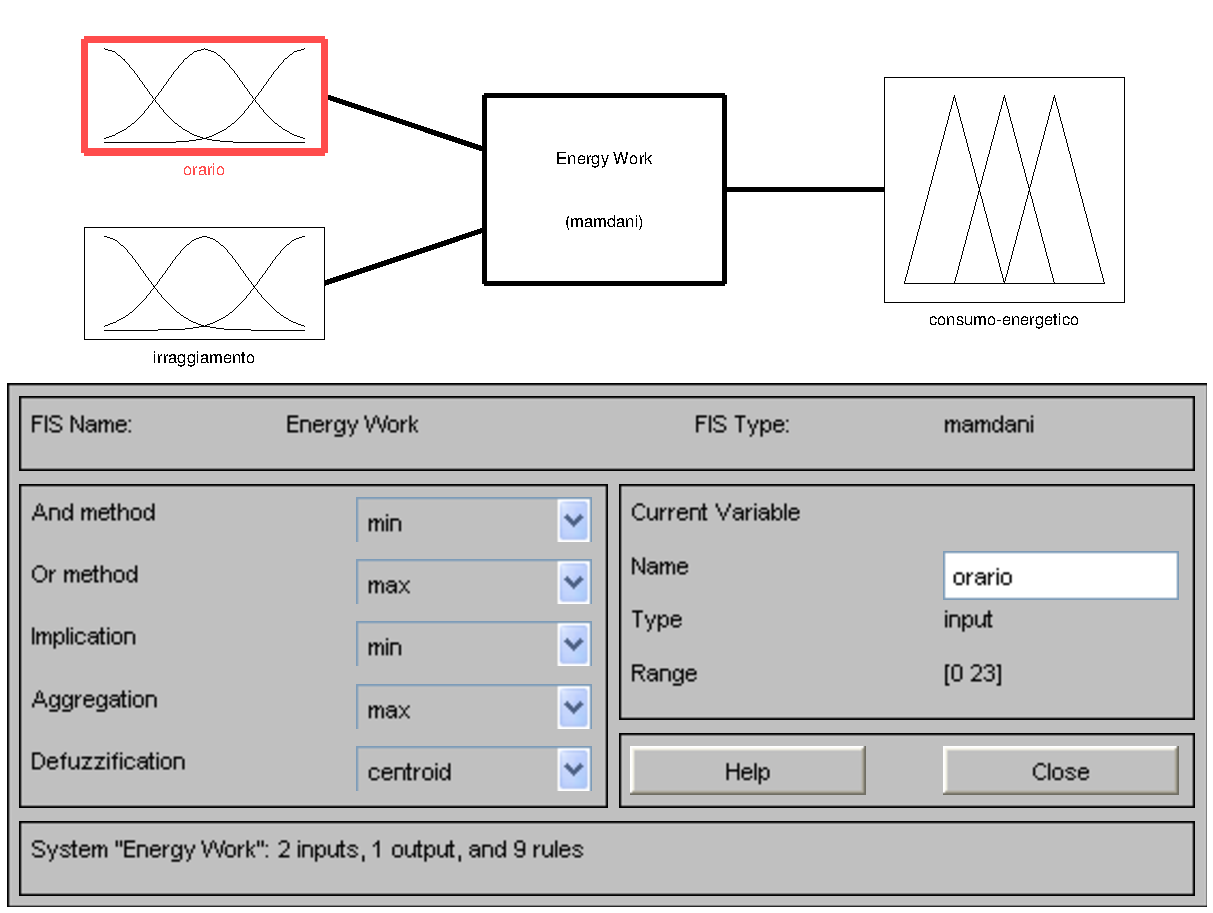
\includegraphics[scale=0.5]{images/fuzzy/modello_fuzzy.pdf}
  \caption{Modello fuzzy}
\end{figure}

\begin{figure}[htbp]
  \centering
  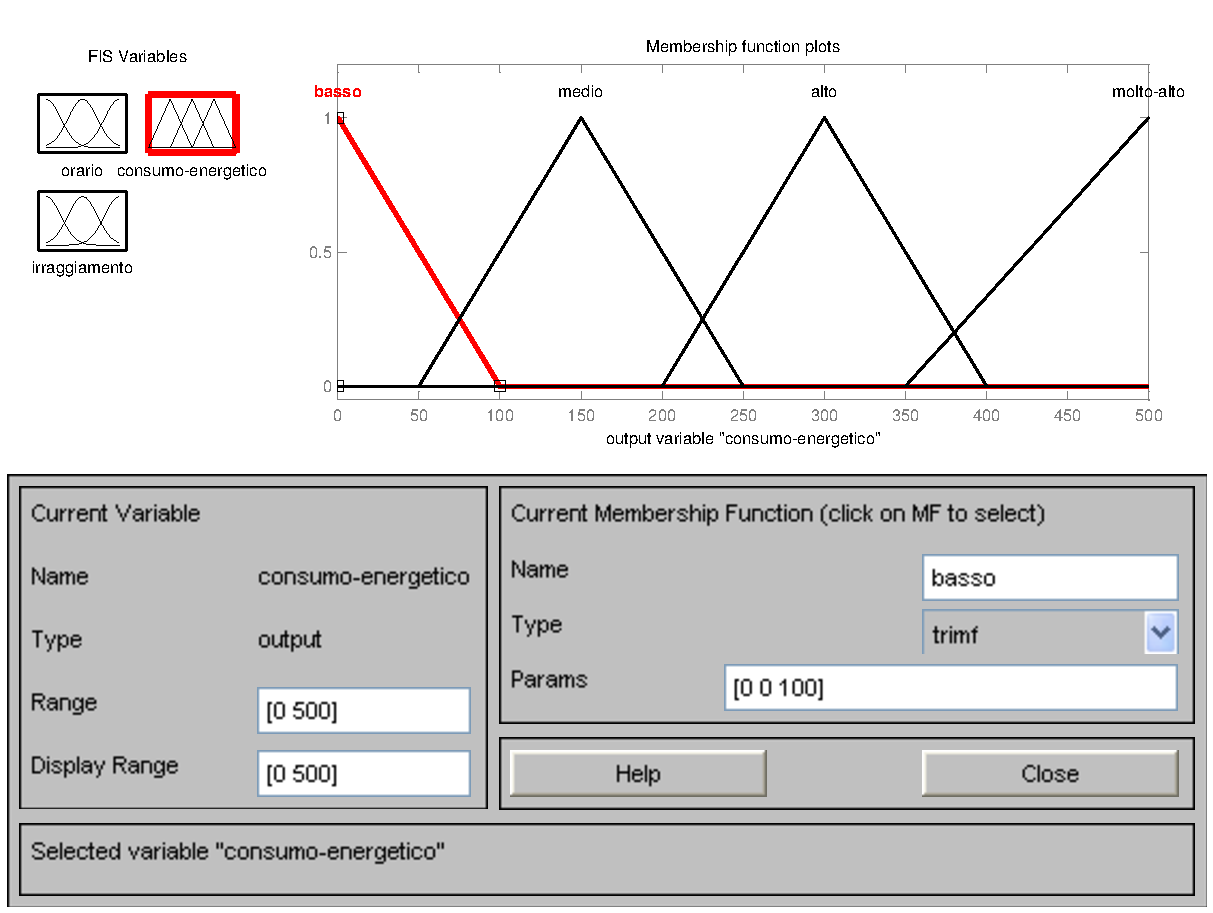
\includegraphics[scale=0.5]{images/fuzzy/variabile_consumo_energetico.pdf}
  \caption{Variabile consumo energetico}
\end{figure}

Per lo studio dell'energia nei giorni feriali, effettuando gli stessi ragionamenti e seguendo la procedura appena descritta otteniamo:
\begin{figure}[htbp]
  \centering
  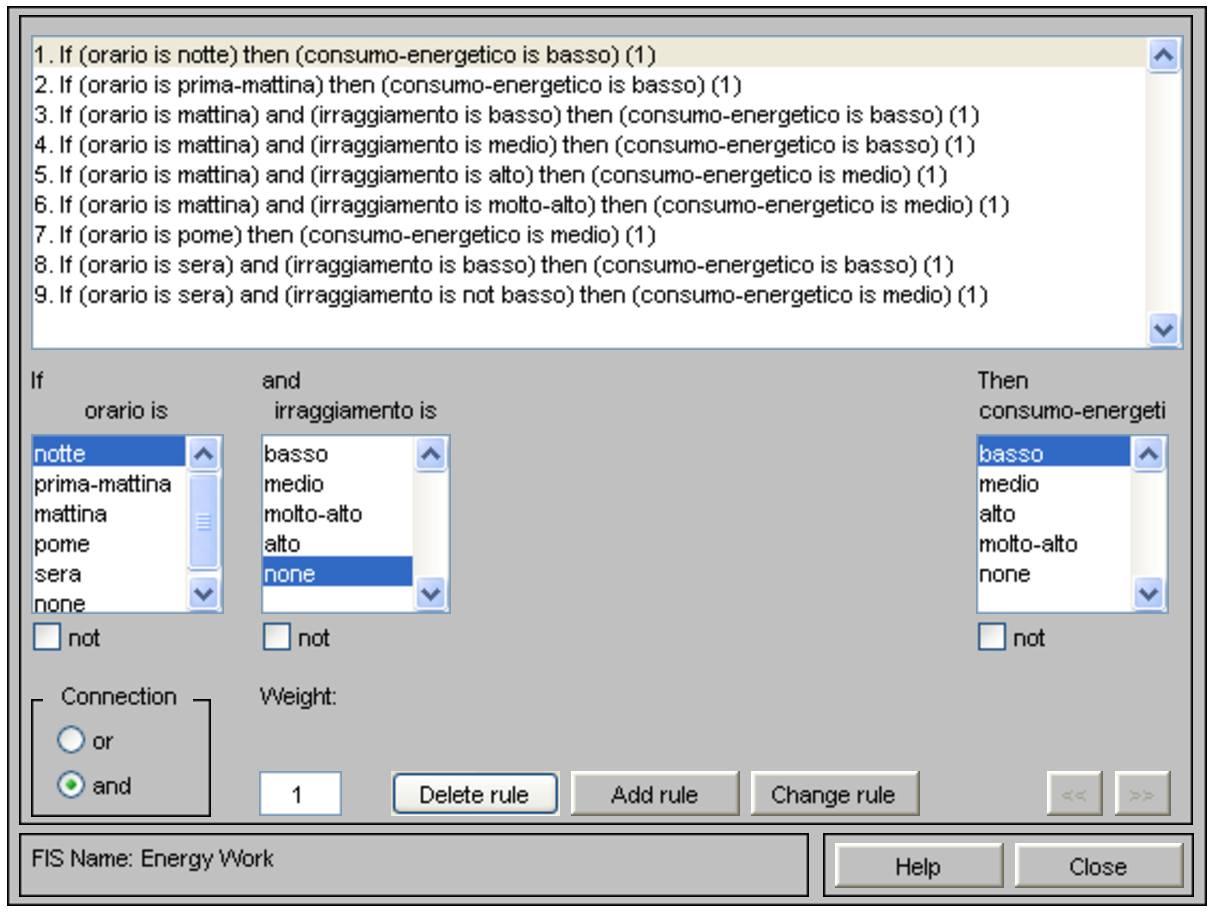
\includegraphics[scale=0.5]{images/fuzzy/energia_feriali_regole.pdf}
  \caption{Energia feriali: regole}
\end{figure}

\begin{figure}[htbp]
  \centering
  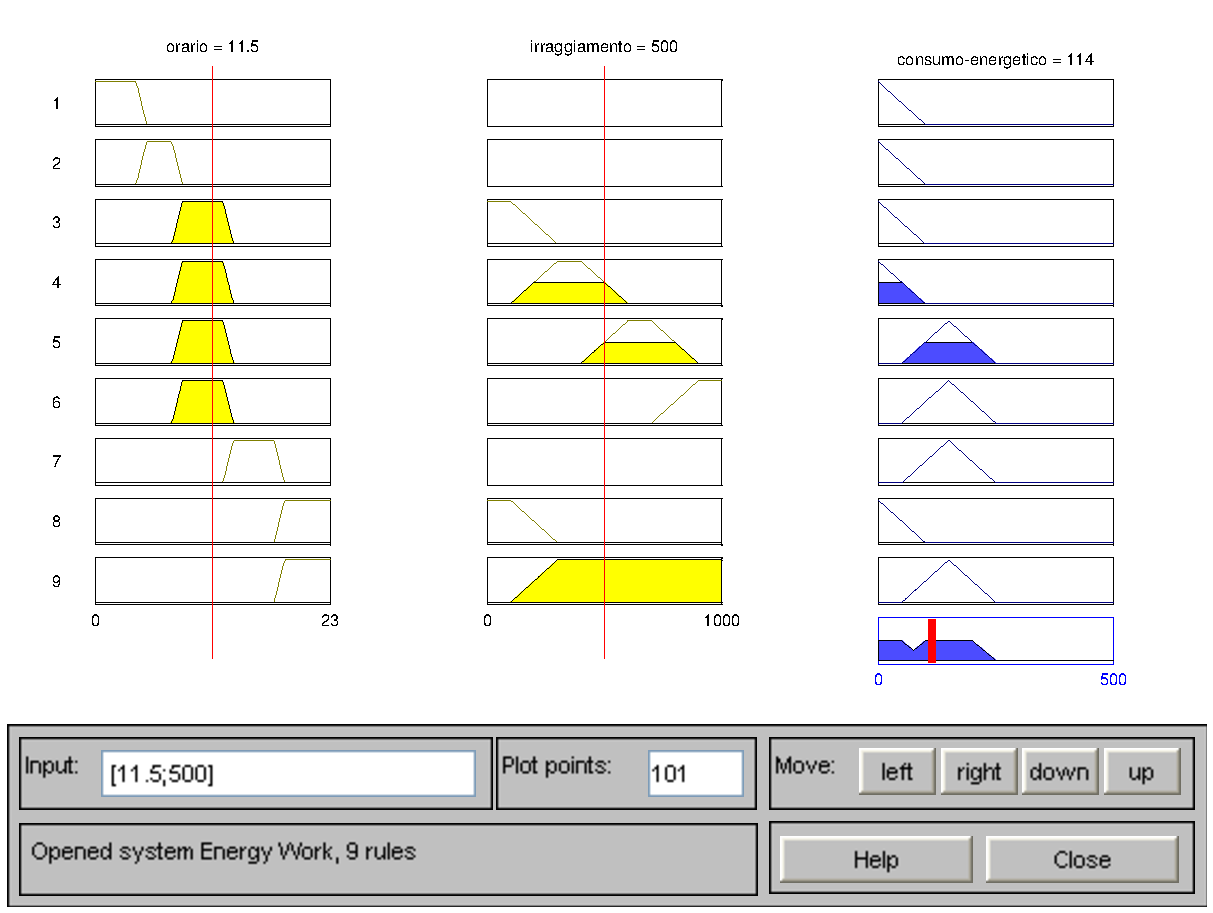
\includegraphics[scale=0.5]{images/fuzzy/energia_feriali_rule_view.pdf}
  \caption{Energia feriali: rule view}
\end{figure}

\begin{figure}[htbp]
  \centering
  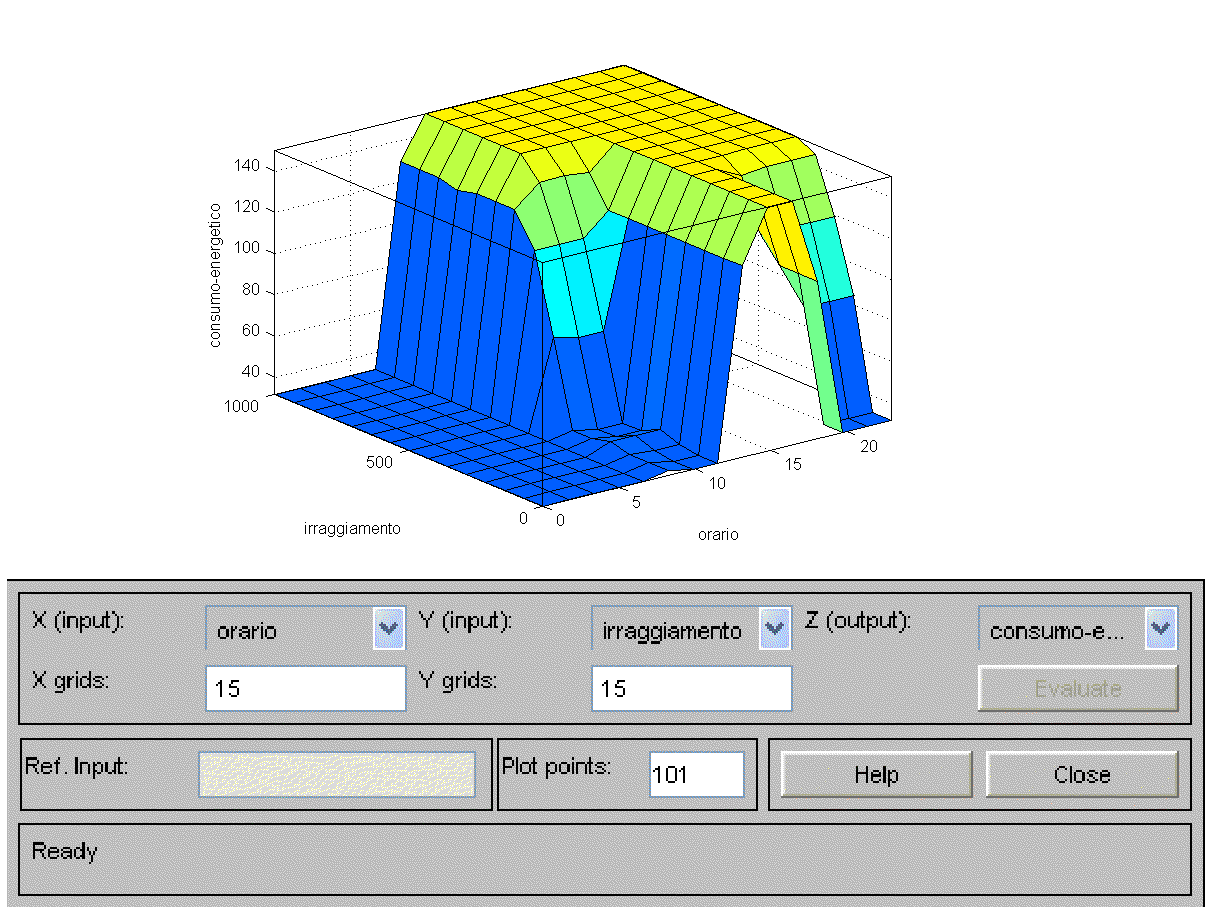
\includegraphics[scale=0.5]{images/fuzzy/energia_feriali_surface_view.pdf}
  \caption{Energia feriali: surface view}
\end{figure}

\begin{table}
  \caption{Risultati}
  \centering
	\begin{tabular}{lr}
		\toprule
      \# di Entry & $ 1005 $ \\
			\# di Hit   & $ 781 $ \\
		\midrule
			& $ 78\% $ \\
		\bottomrule
	\end{tabular}
\end{table}


\subsubsection{Luminosità - Festivi}

\begin{figure}[htbp]
  \centering
  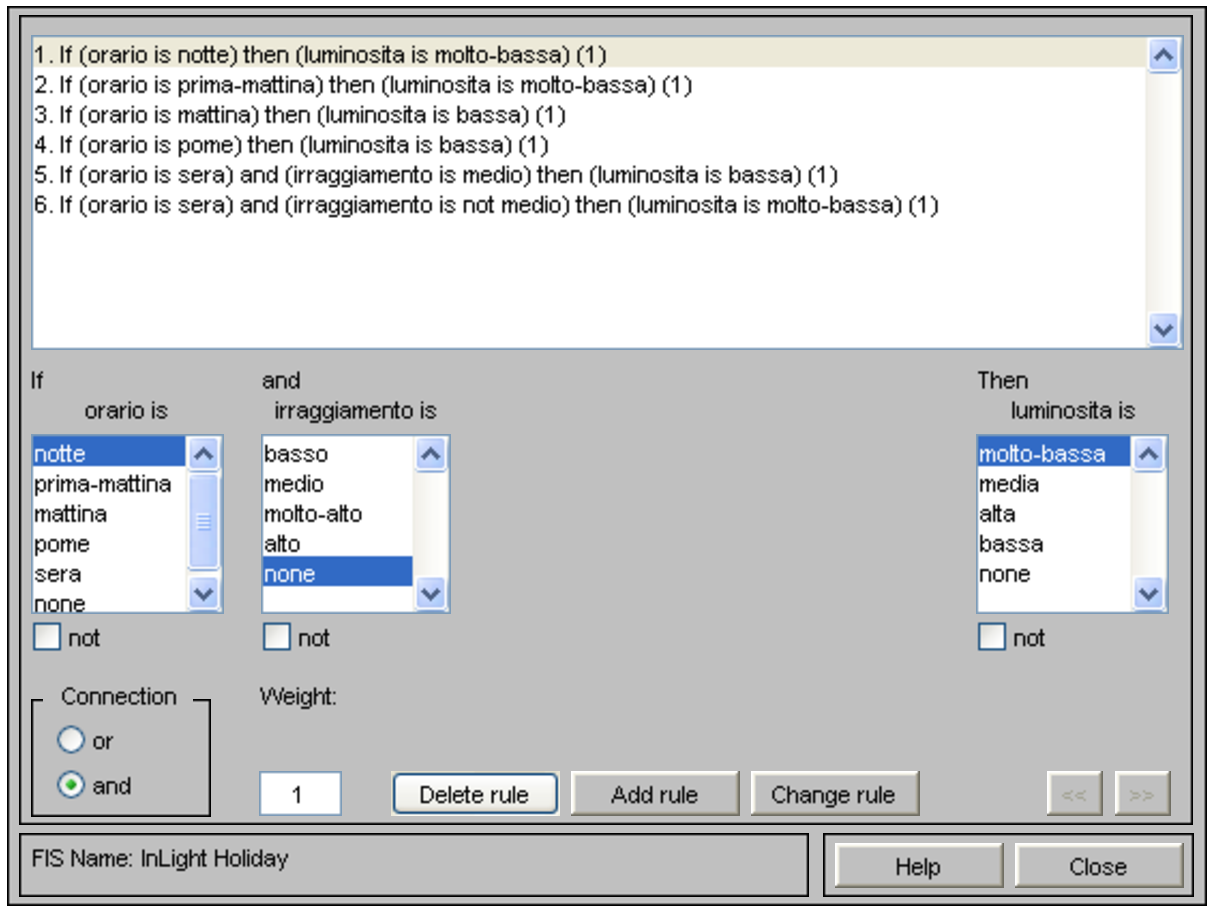
\includegraphics[scale=0.5]{images/fuzzy/luminosita_festivi_regole.pdf}
  \caption{Luminosità festivi: regole}
\end{figure}

\begin{figure}[htbp]
  \centering
  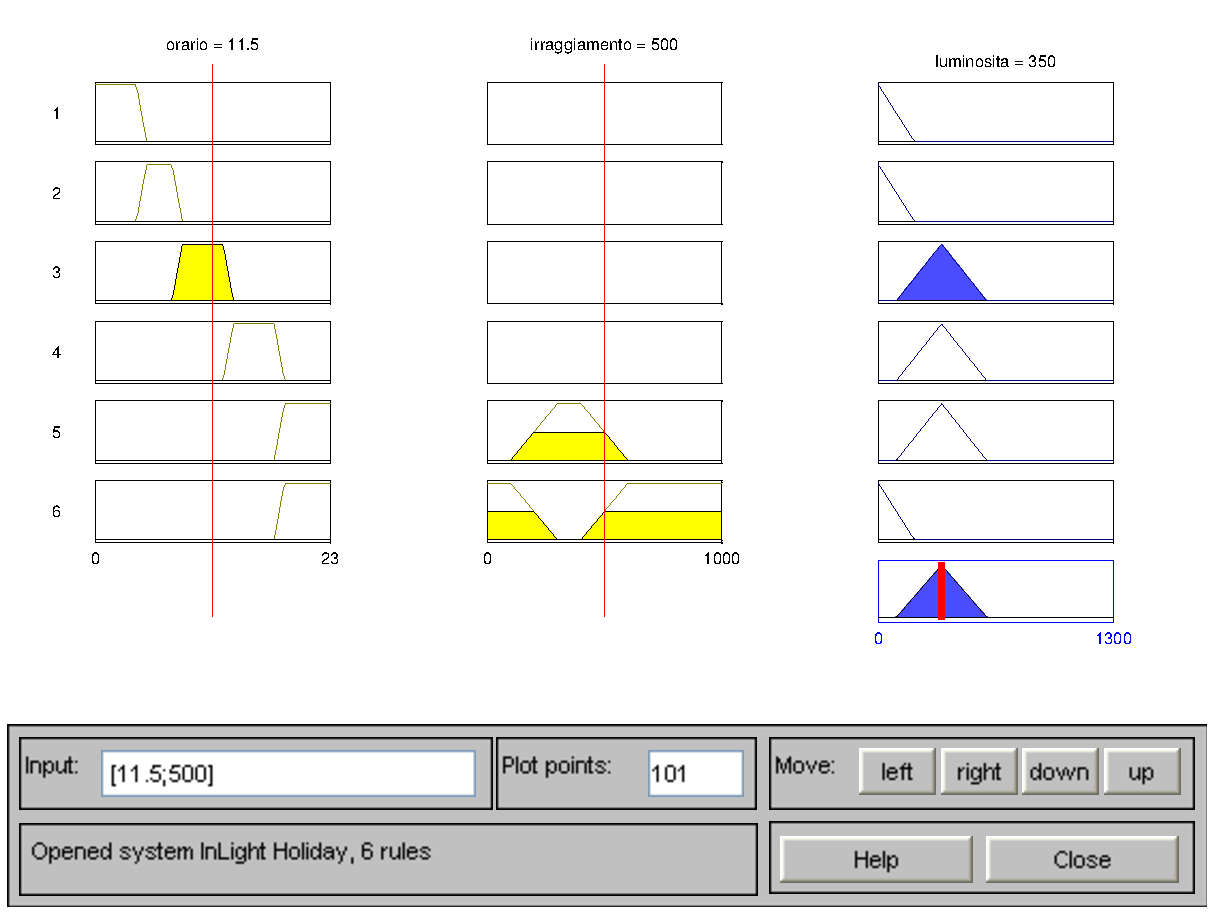
\includegraphics[scale=0.5]{images/fuzzy/luminosita_festivi_rule_view.pdf}
  \caption{Luminosità festivi: rule view}
\end{figure}

\begin{figure}[htbp]
  \centering
  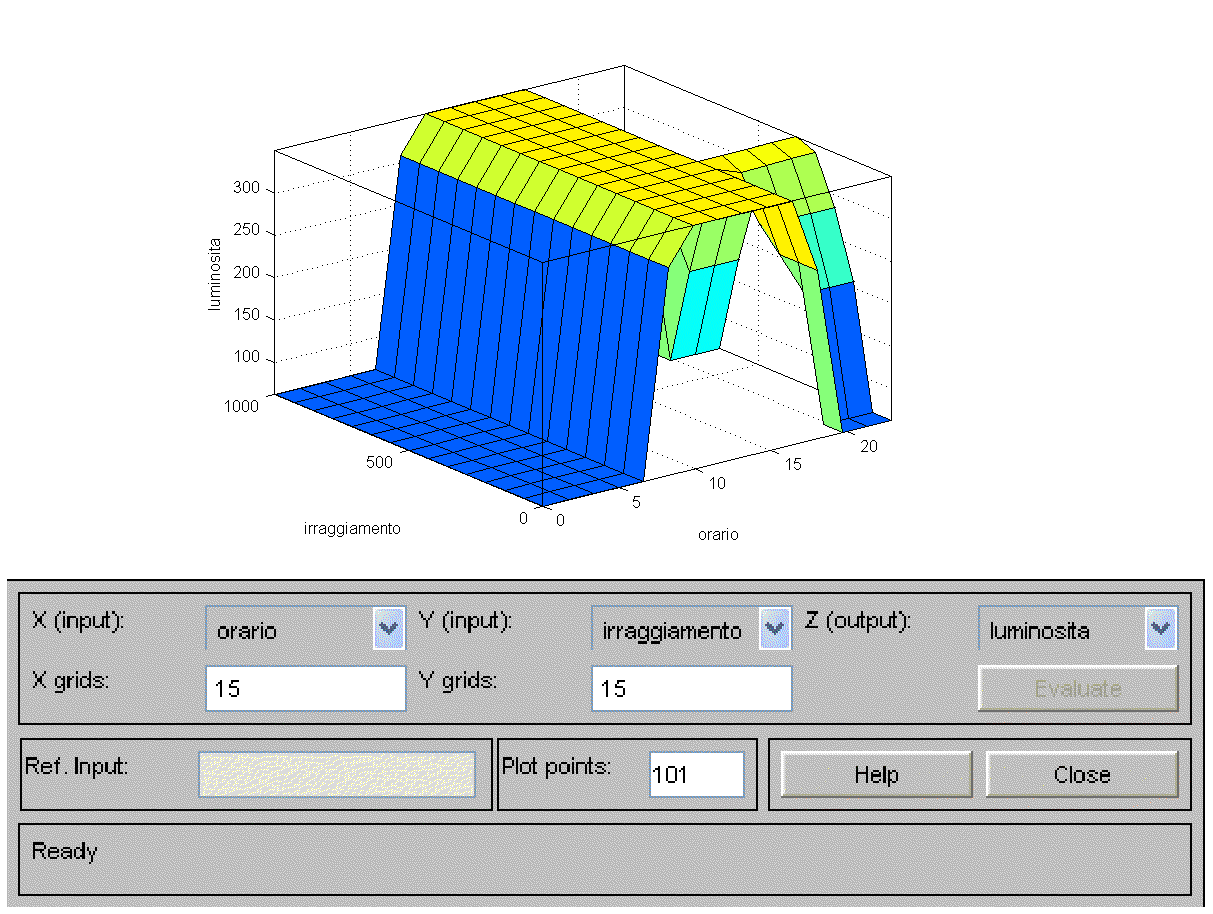
\includegraphics[scale=0.5]{images/fuzzy/luminosita_festivi_surface_view.pdf}
  \caption{Luminosità festivi: surface view}
\end{figure}

\begin{table}
  \caption{Risultati}
  \centering
	\begin{tabular}{lr}
		\toprule
      \# di Entry & $ 528 $ \\
			\# di Hit   & $ 436 $ \\
		\midrule
			& $ 83\% $ \\
		\bottomrule
	\end{tabular}
\end{table}


\subsubsection{Energia - Festivi}

\begin{figure}[htbp]
  \centering
  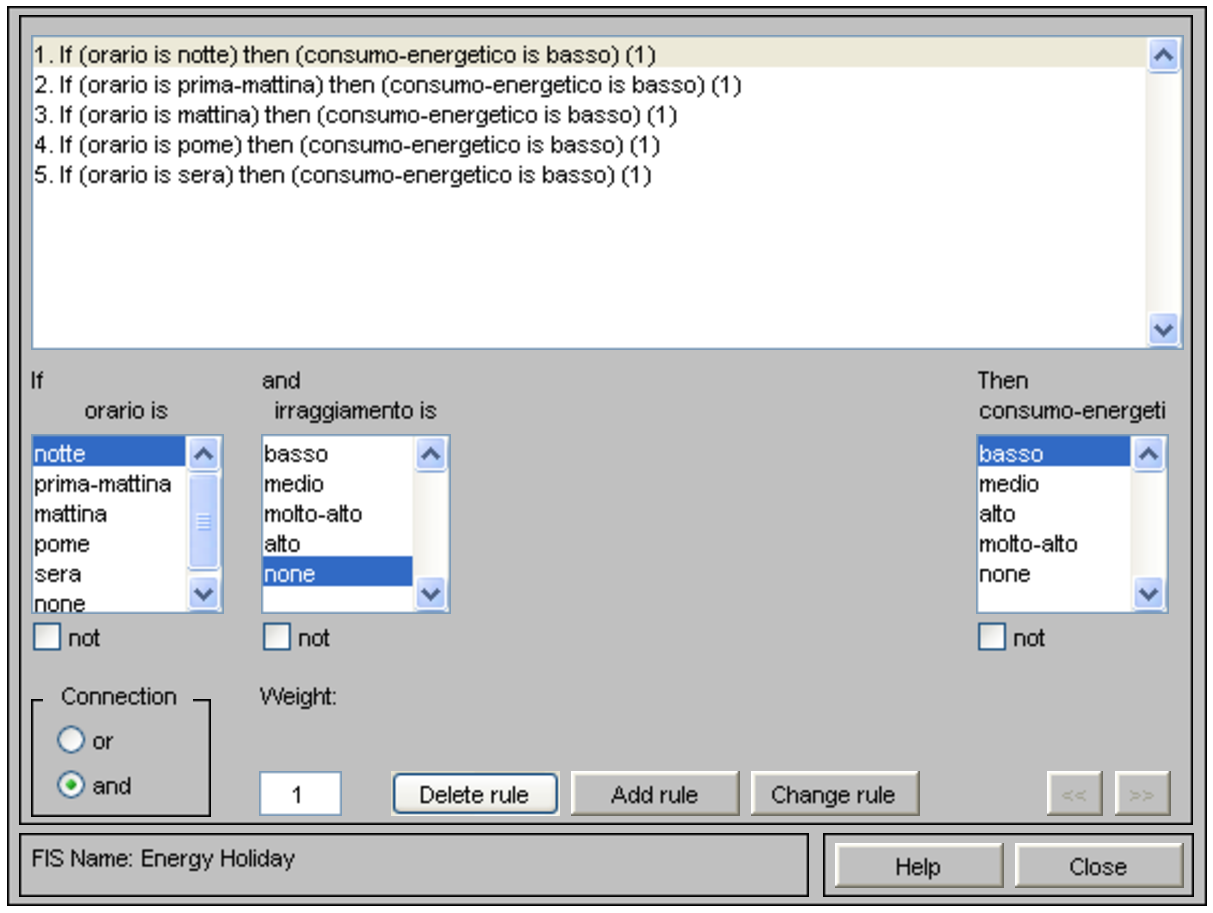
\includegraphics[scale=0.5]{images/fuzzy/energia_festivi_regole.pdf}
  \caption{Energia festivi: regole}
\end{figure}

\begin{figure}[htbp]
  \centering
  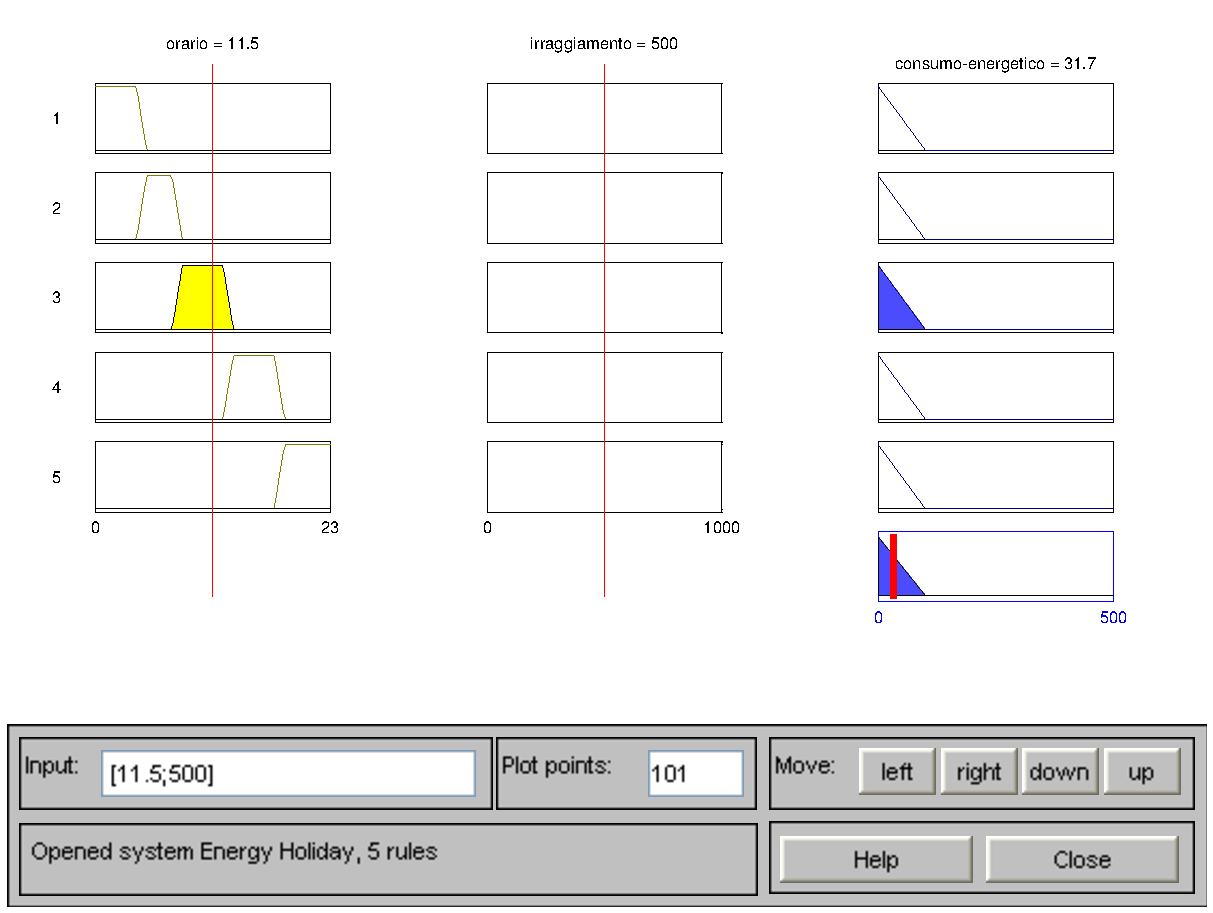
\includegraphics[scale=0.5]{images/fuzzy/energia_festivi_rule_view.pdf}
  \caption{Energia festivi: rule view}
\end{figure}

\begin{figure}[htbp]
  \centering
  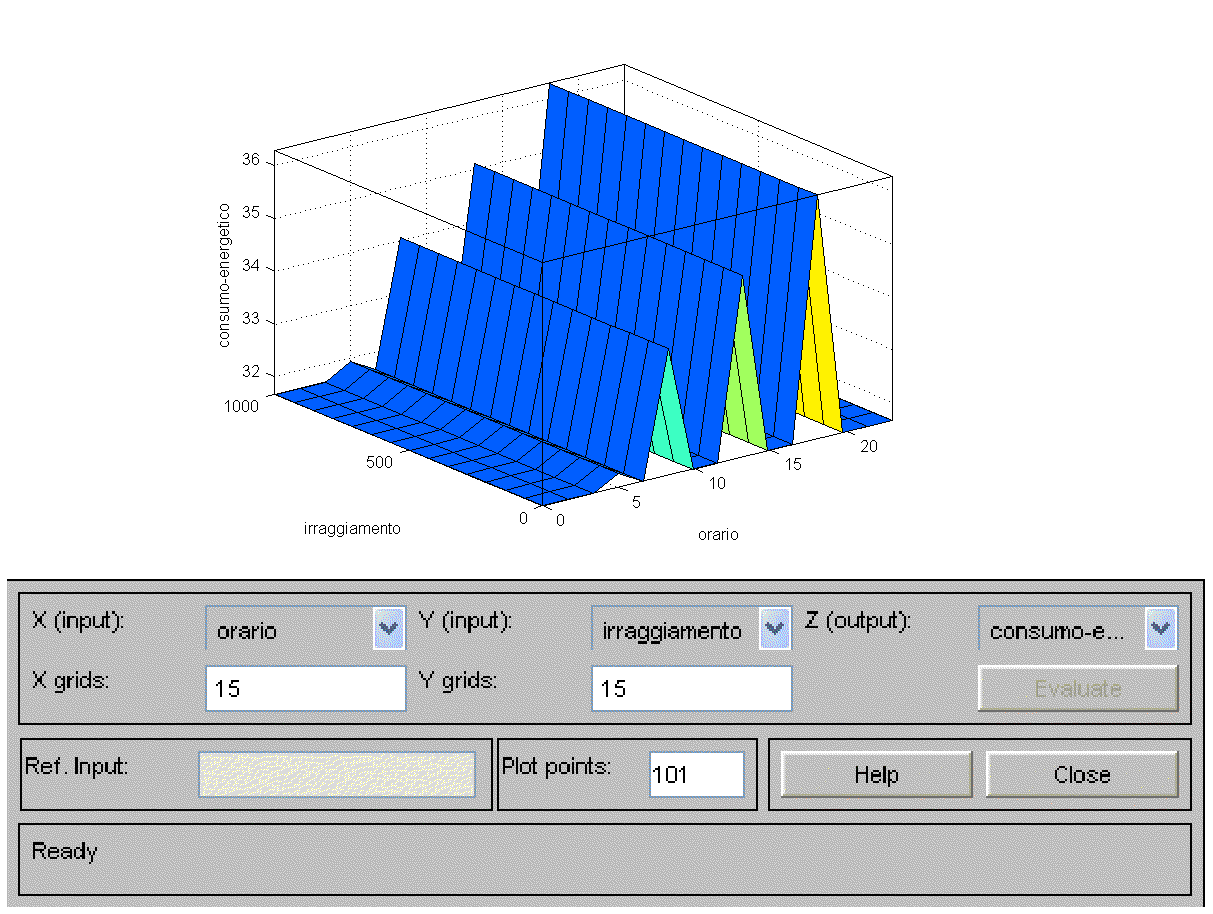
\includegraphics[scale=0.5]{images/fuzzy/energia_festivi_surface_view.pdf}
  \caption{Energia festivi: surface view}
\end{figure}

\begin{table}
  \caption{Risultati}
  \centering
	\begin{tabular}{lr}
		\toprule
      \# di Entry & $ 528 $ \\
			\# di Hit   & $ 491 $ \\
		\midrule
			& $ 93\% $ \\
		\bottomrule
	\end{tabular}
\end{table}

\clearpage
